% Slide 1: Quick Overview
\begin{frame}{Quick Overview}
    \begin{itemize}
        \item Wet dry sensor validation
        \item 3-axis acceleration and offset
        \item Temperature sensor data
        \item Key insights
    \end{itemize}
\end{frame}


% Slide 2: Wet Dry Sensor Validation
\begin{frame}{Wet Dry Sensor Validation}
    \begin{figure}
        \centering
        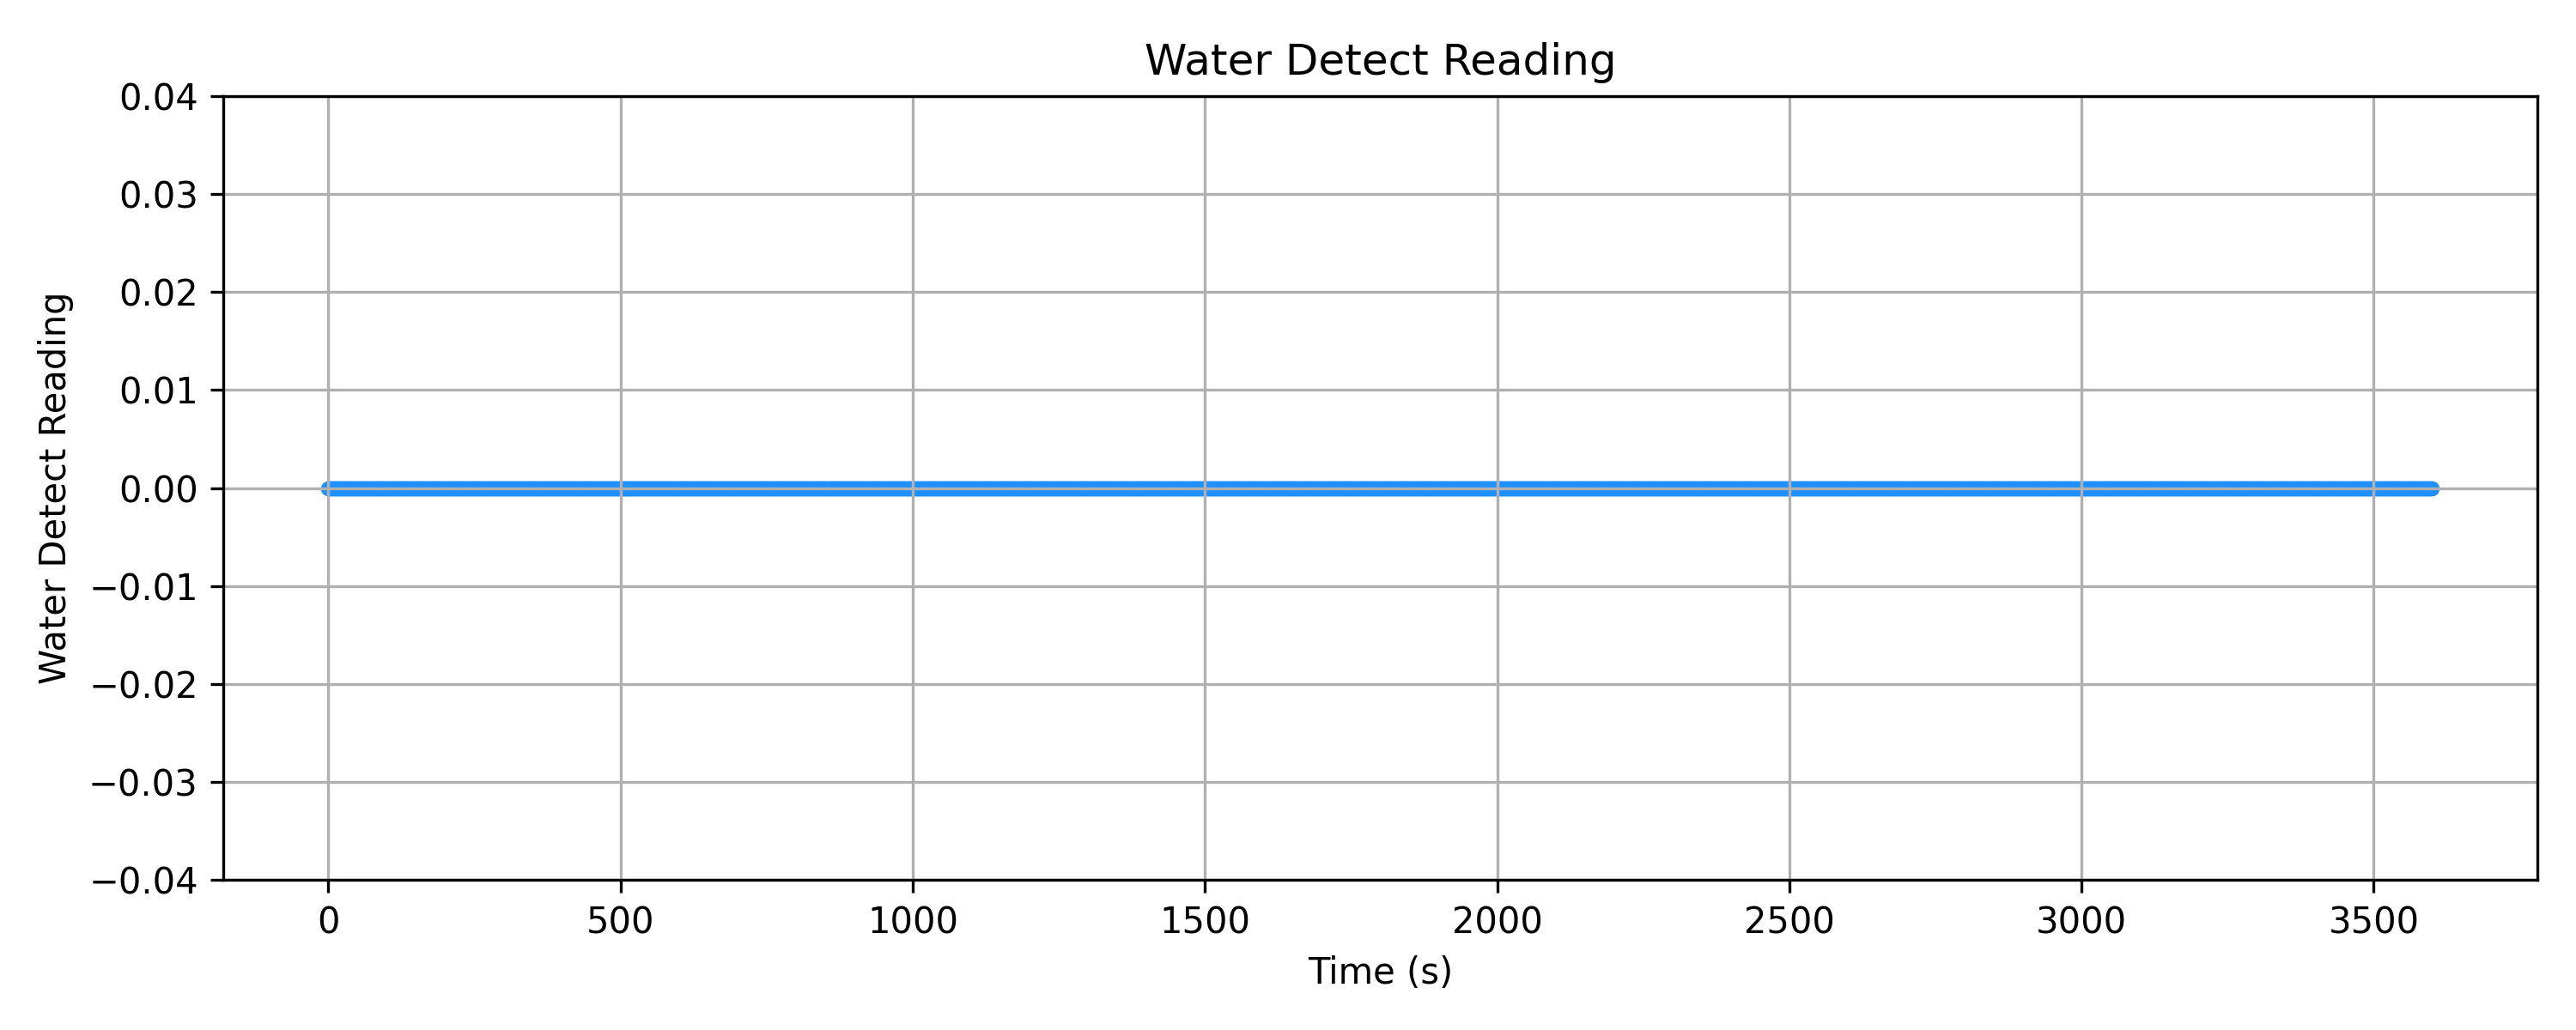
\includegraphics[height=1.1\textheight,width=0.8\textwidth,keepaspectratio]{images/water_detect.png}
    \end{figure}
        \begin{itemize} 
            \item Perfect dry-state detection
            \item Consistent 0.000 readings
            \item No false positives
        \end{itemize}
\end{frame}

% Slide 3: Vertical Acceleration
\begin{frame}{Accelerations}
    \begin{columns}[onlytextwidth]
        \begin{column}{0.46\textwidth}
            \vspace{0.5em}
            \hspace{-2em}
            \begin{figure}
                \centering
                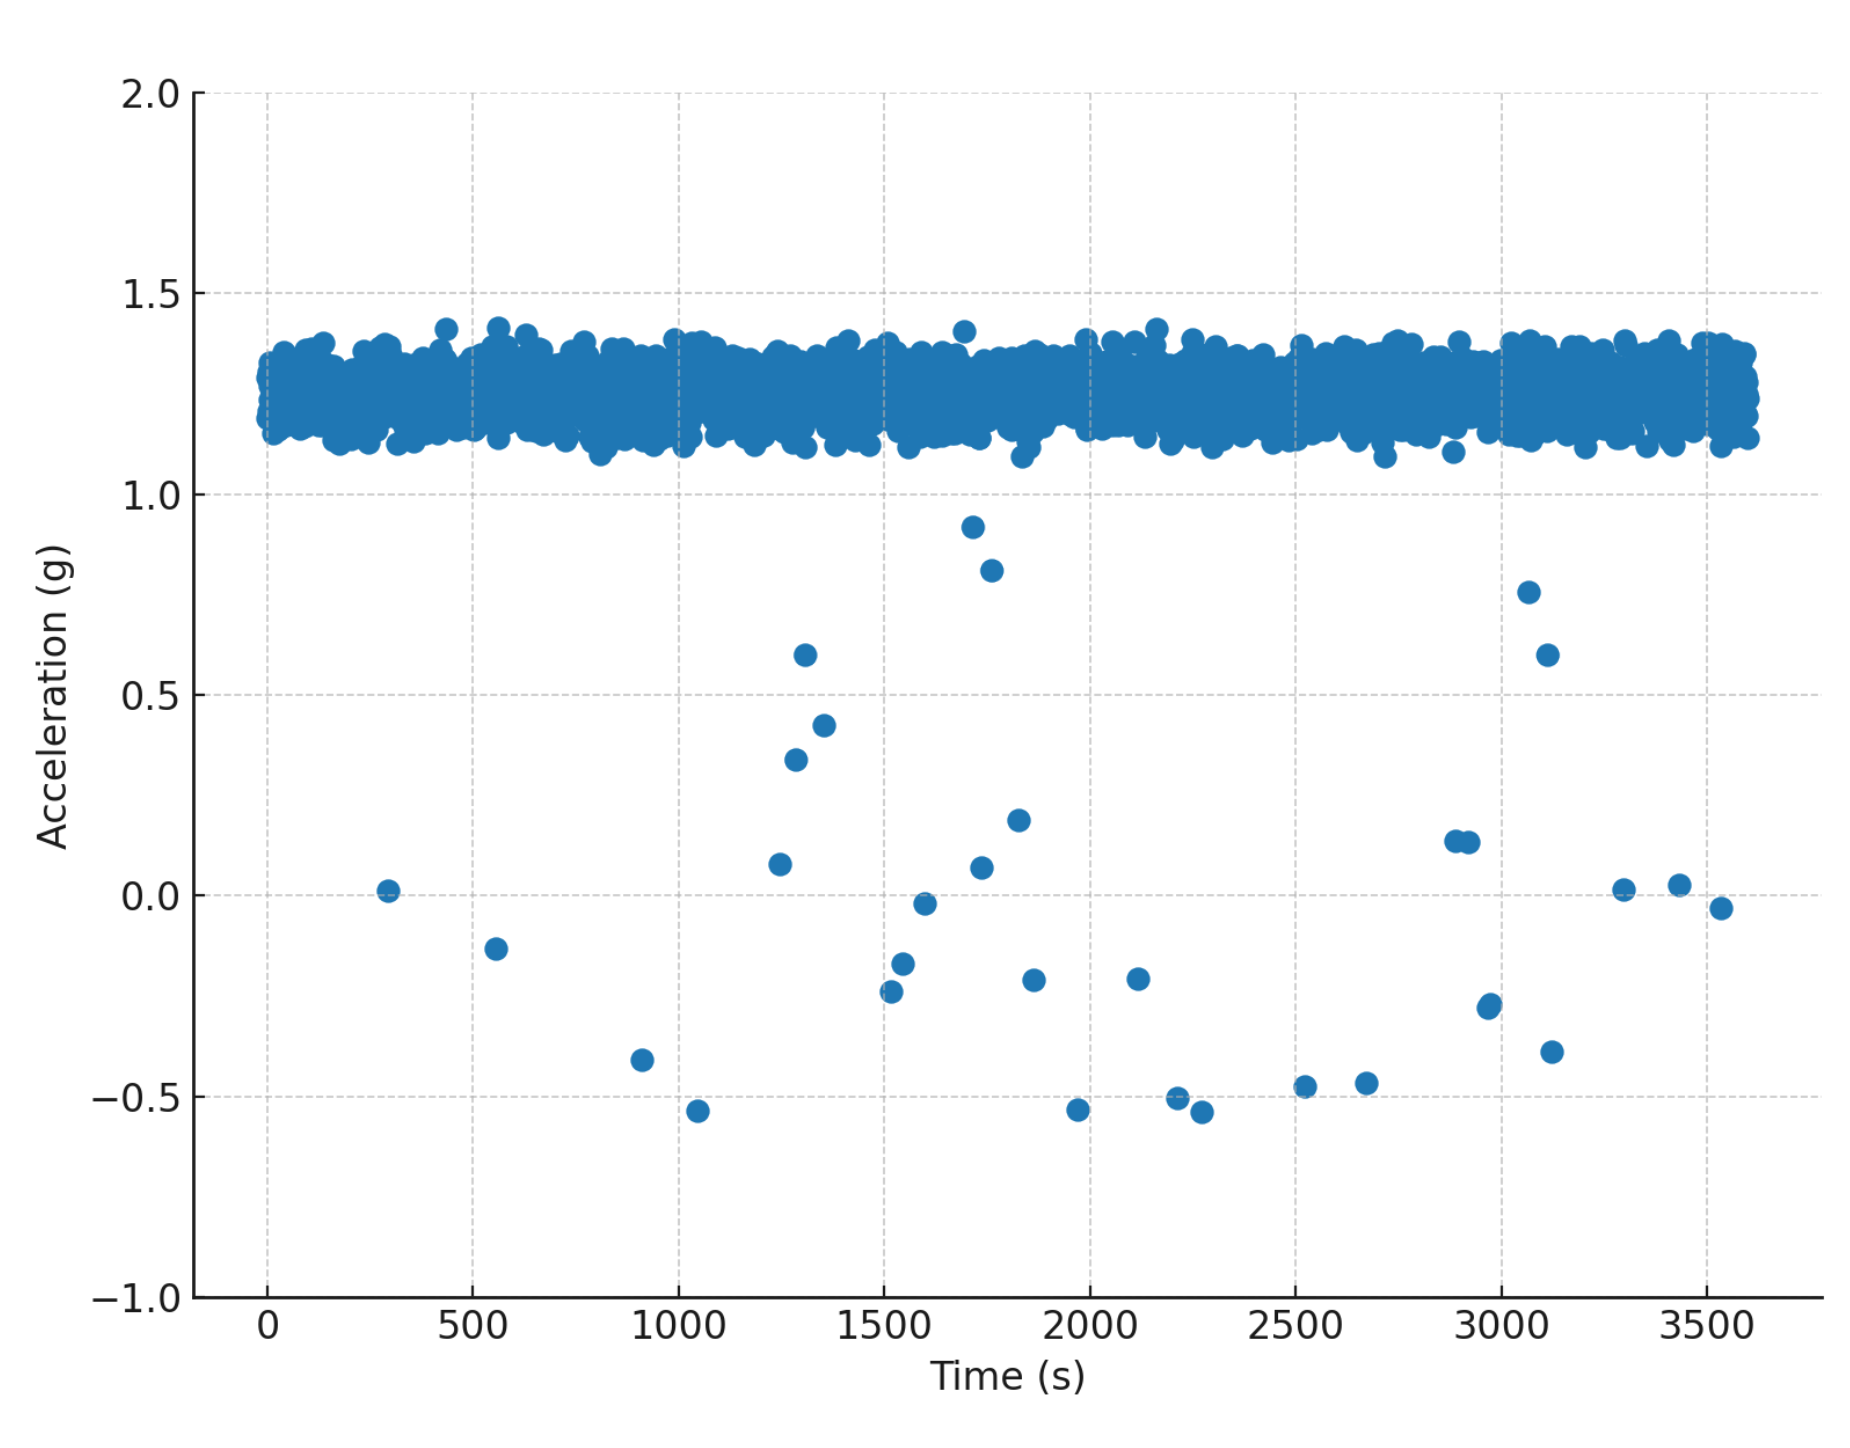
\includegraphics[height=0.6\textheight,width=1.05\textwidth,keepaspectratio]{images/z_acceleration.png}
                \caption{Z-axis acceleration}
            \end{figure}
        \end{column}

        \begin{column}{0.54\textwidth}
            \vspace{-0.3em}
            \begin{figure}
                \centering
                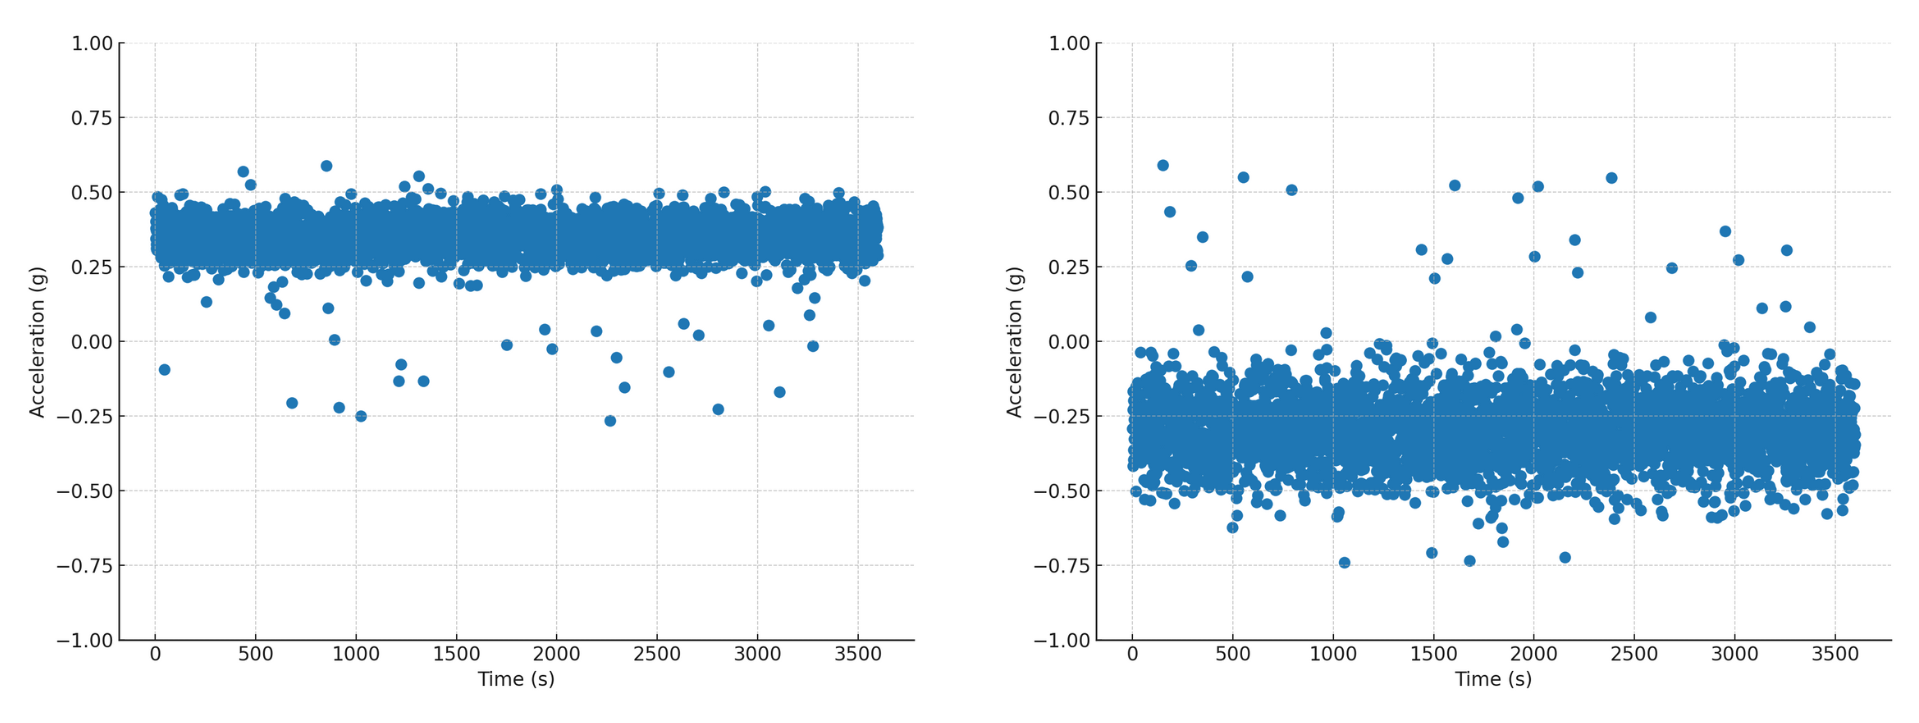
\includegraphics[height=0.4\textheight,width=1.1\textwidth,keepaspectratio]{images/xy-axis-acceleration.png}
                \caption{Y and X axis accelerations}
            \end{figure}
            \vspace{-1.8em} 
            \begin{figure}
                \centering
                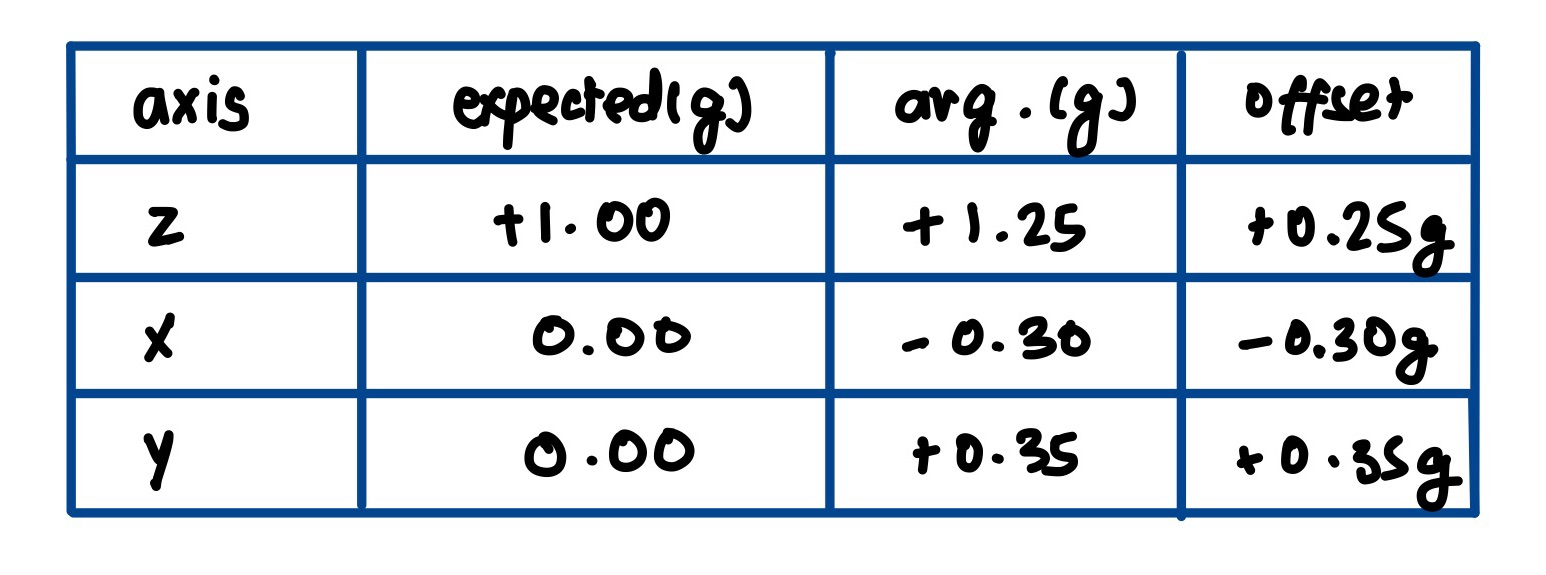
\includegraphics[height=0.25\textheight,width=0.9\textwidth,keepaspectratio]{images/table_axes.jpg}
                \caption{Offset values for the axes}
            \end{figure}
        \end{column}
    \end{columns}
\end{frame}


% Slide 4: Temperature Over Time
\begin{frame}{Temperature Sensor Over Time}
    \begin{figure}
        \centering
        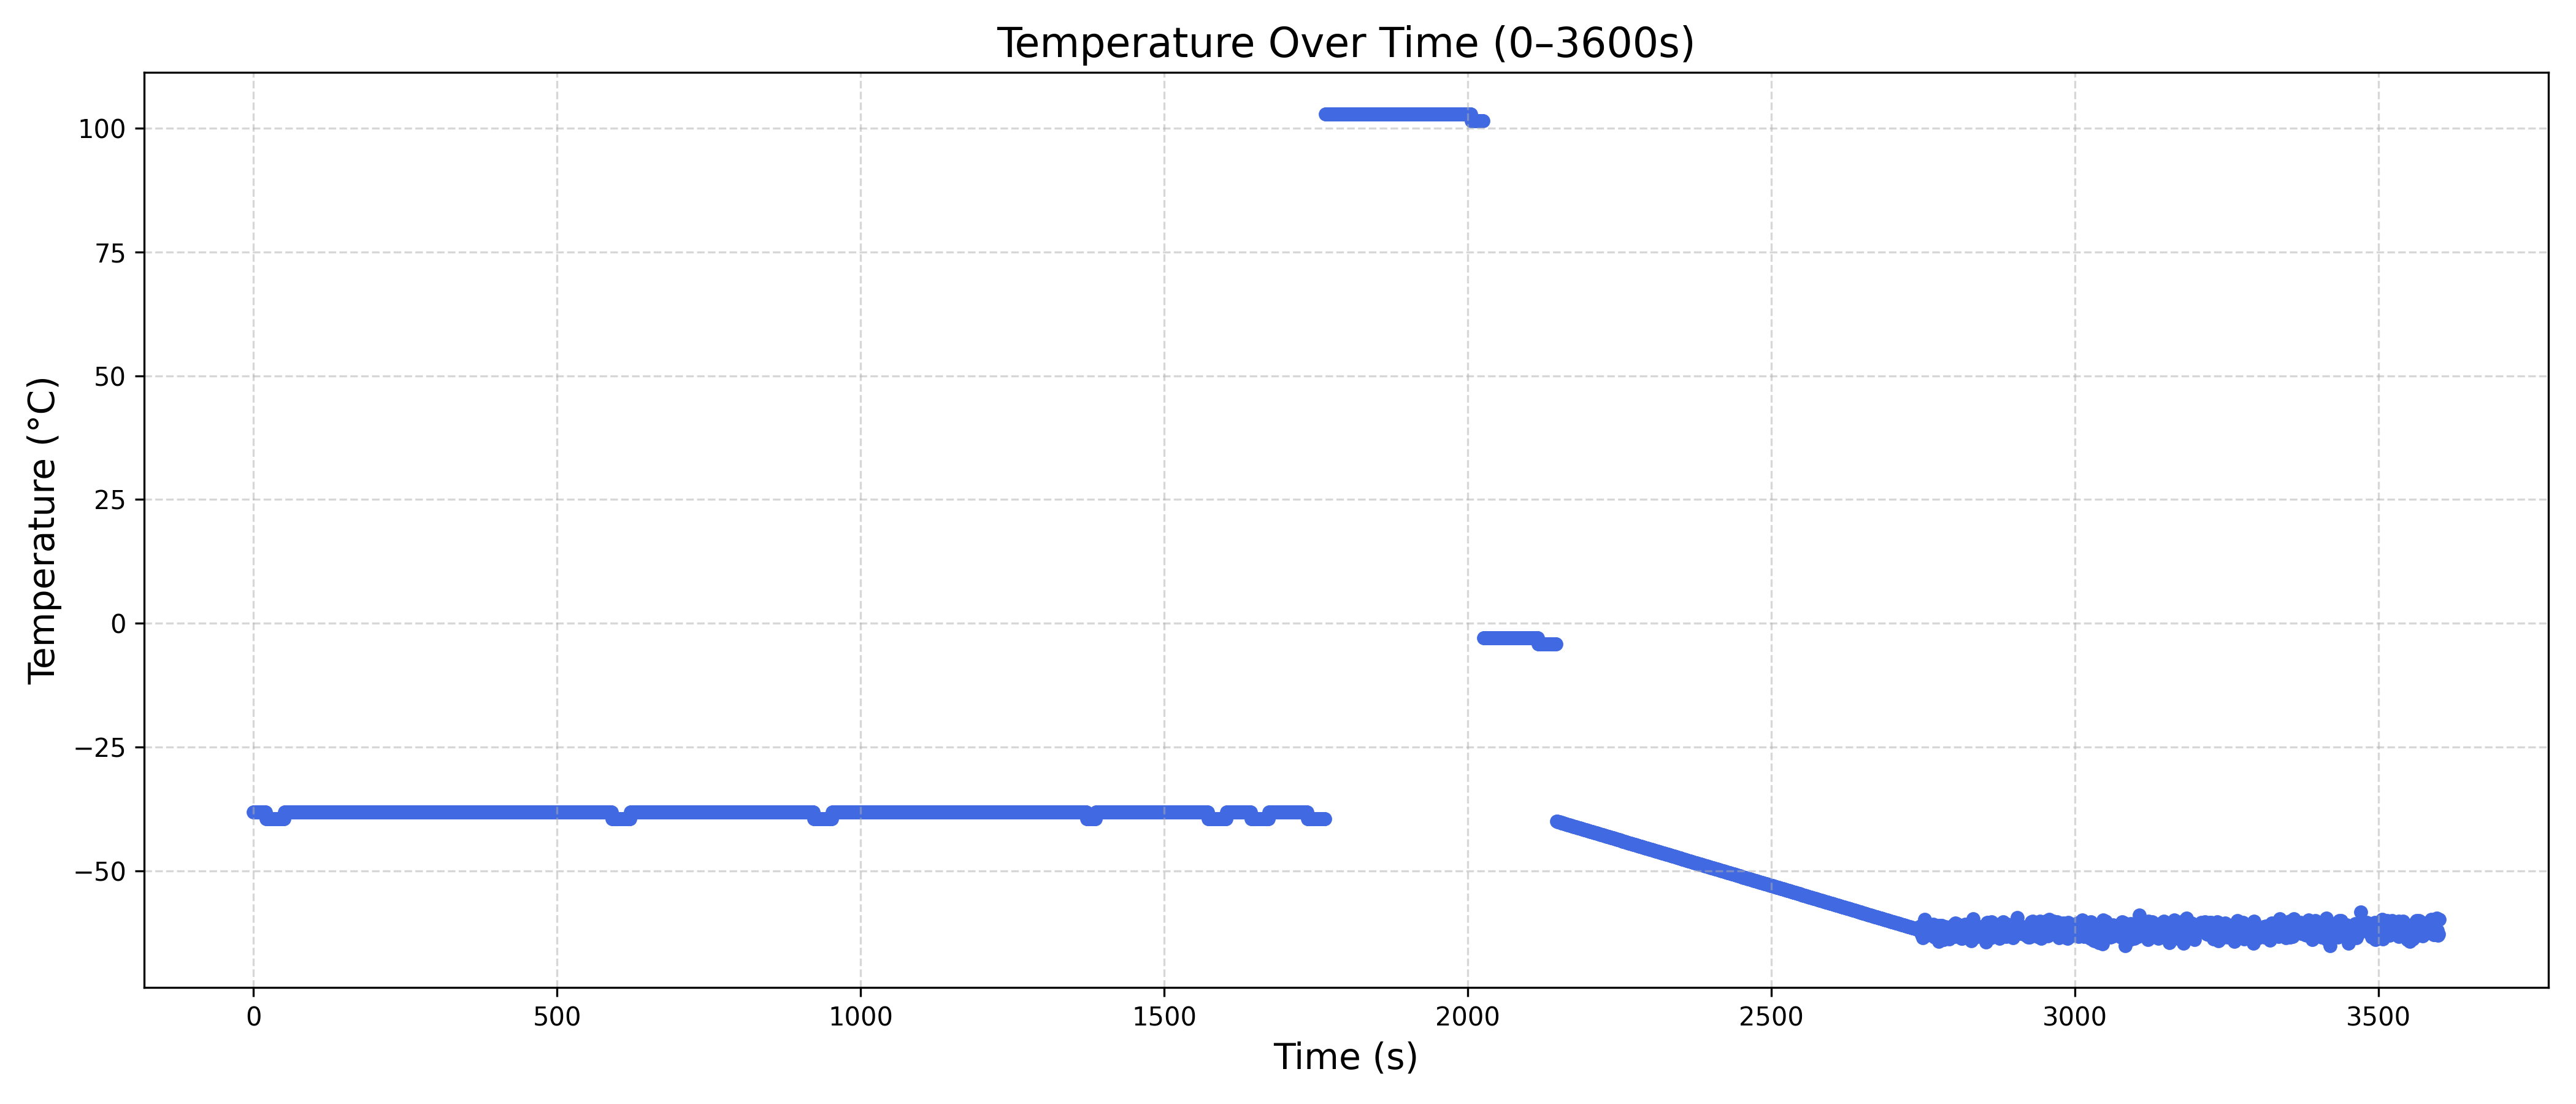
\includegraphics[height=0.5\textheight,width=0.9\textwidth,keepaspectratio]{images/temp_over_time.png}
        \caption{Temperature over time}
    \end{figure}
    \vspace{-1em}
    \begin{itemize}
        \item Inconsistent data
        \item Heavily negative temperature values
        \item Sudden peak at 100°C is highly suspicious
    \end{itemize}
\end{frame}

% Slide 5: Temperature Histogram
\begin{frame}{Frequency Histogram}
    \begin{figure}
        \centering
        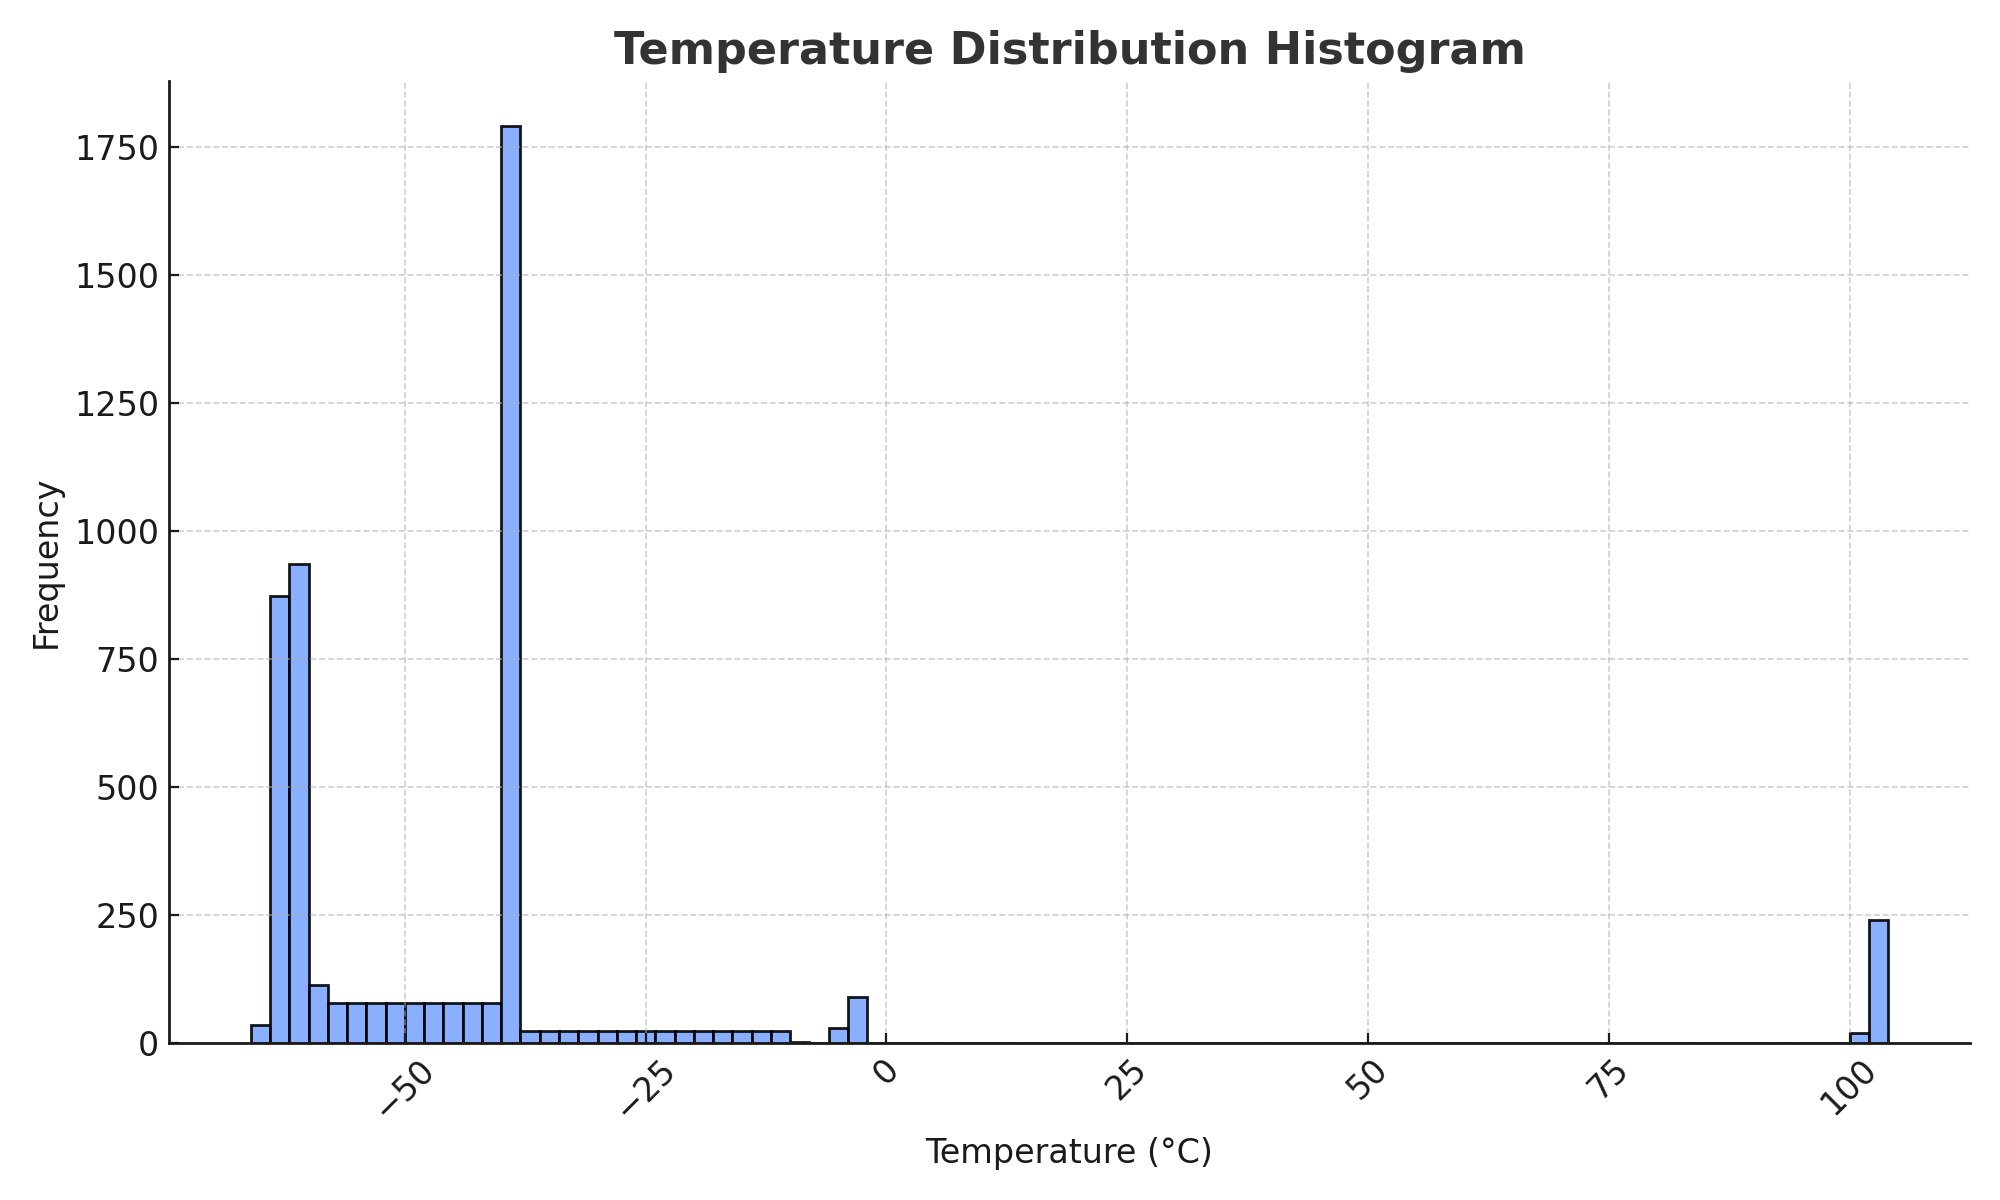
\includegraphics[height=0.6\textheight,width=0.95\textwidth,keepaspectratio]{images/temp_histogram.png}
        \caption{Temperature frequency histogram}
    \end{figure}
    \vspace{-0.5em}
    \begin{itemize}
        \item Histogram spikes at  -40°C, 0°C, and 100°C
        \item Many implausible temperatures: likely a formula or decoding issue
    \end{itemize}
\end{frame}

% Slide 6: Next Steps
\begin{frame}{Next Steps}
    \begin{itemize}
        \item Refine temperature decoding logic
        \item Perhaps -- validate with reference thermometer
        \item Salinity tests
        \item Remaining IMU assessment
    \end{itemize}
\end{frame}

\begin{frame}{Hardware Development}
    \centering
    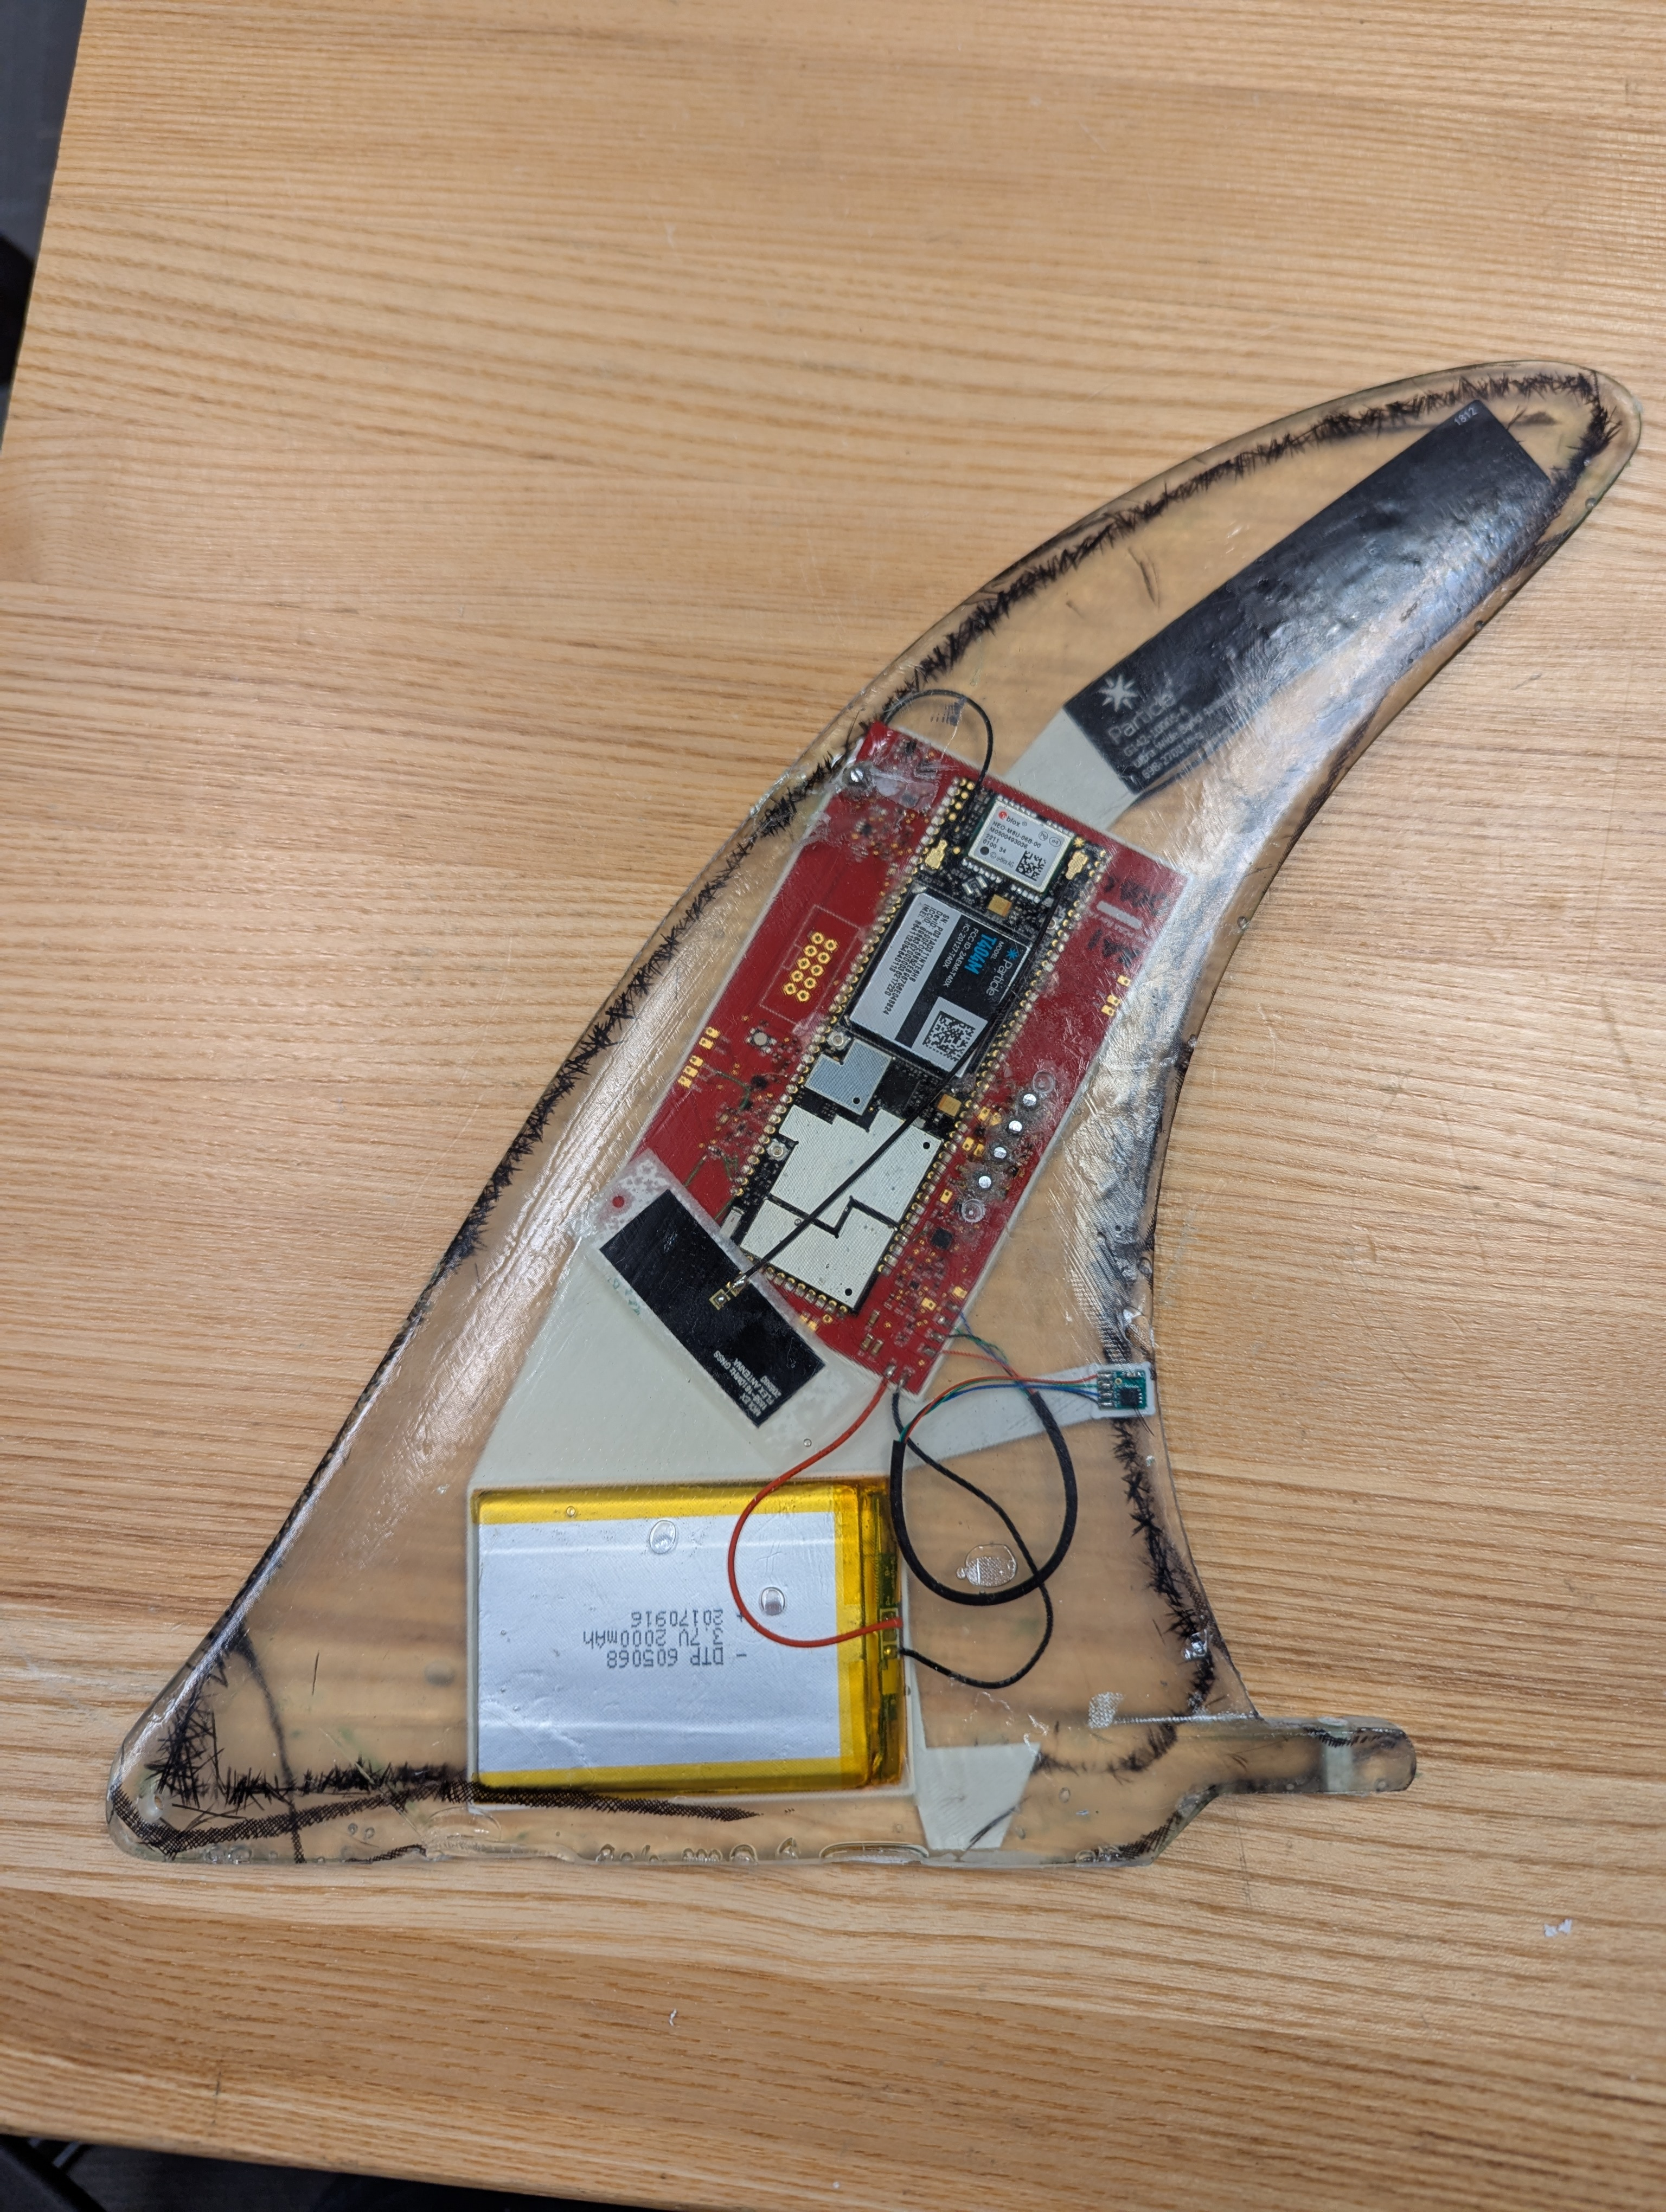
\includegraphics[height=0.6\textheight,width=0.95\textwidth,keepaspectratio]{images/sf_sn0002_complete.jpg}
\end{frame}

\begin{frame}{Issues Discovered}
    \begin{itemize}
        \item Discharged Battery
        \item Charger Sense
        \item Battery Charging
        \item USB Enumeration
    \end{itemize}
\end{frame}

\begin{frame}{Manual Battery Charging}
    \centering
    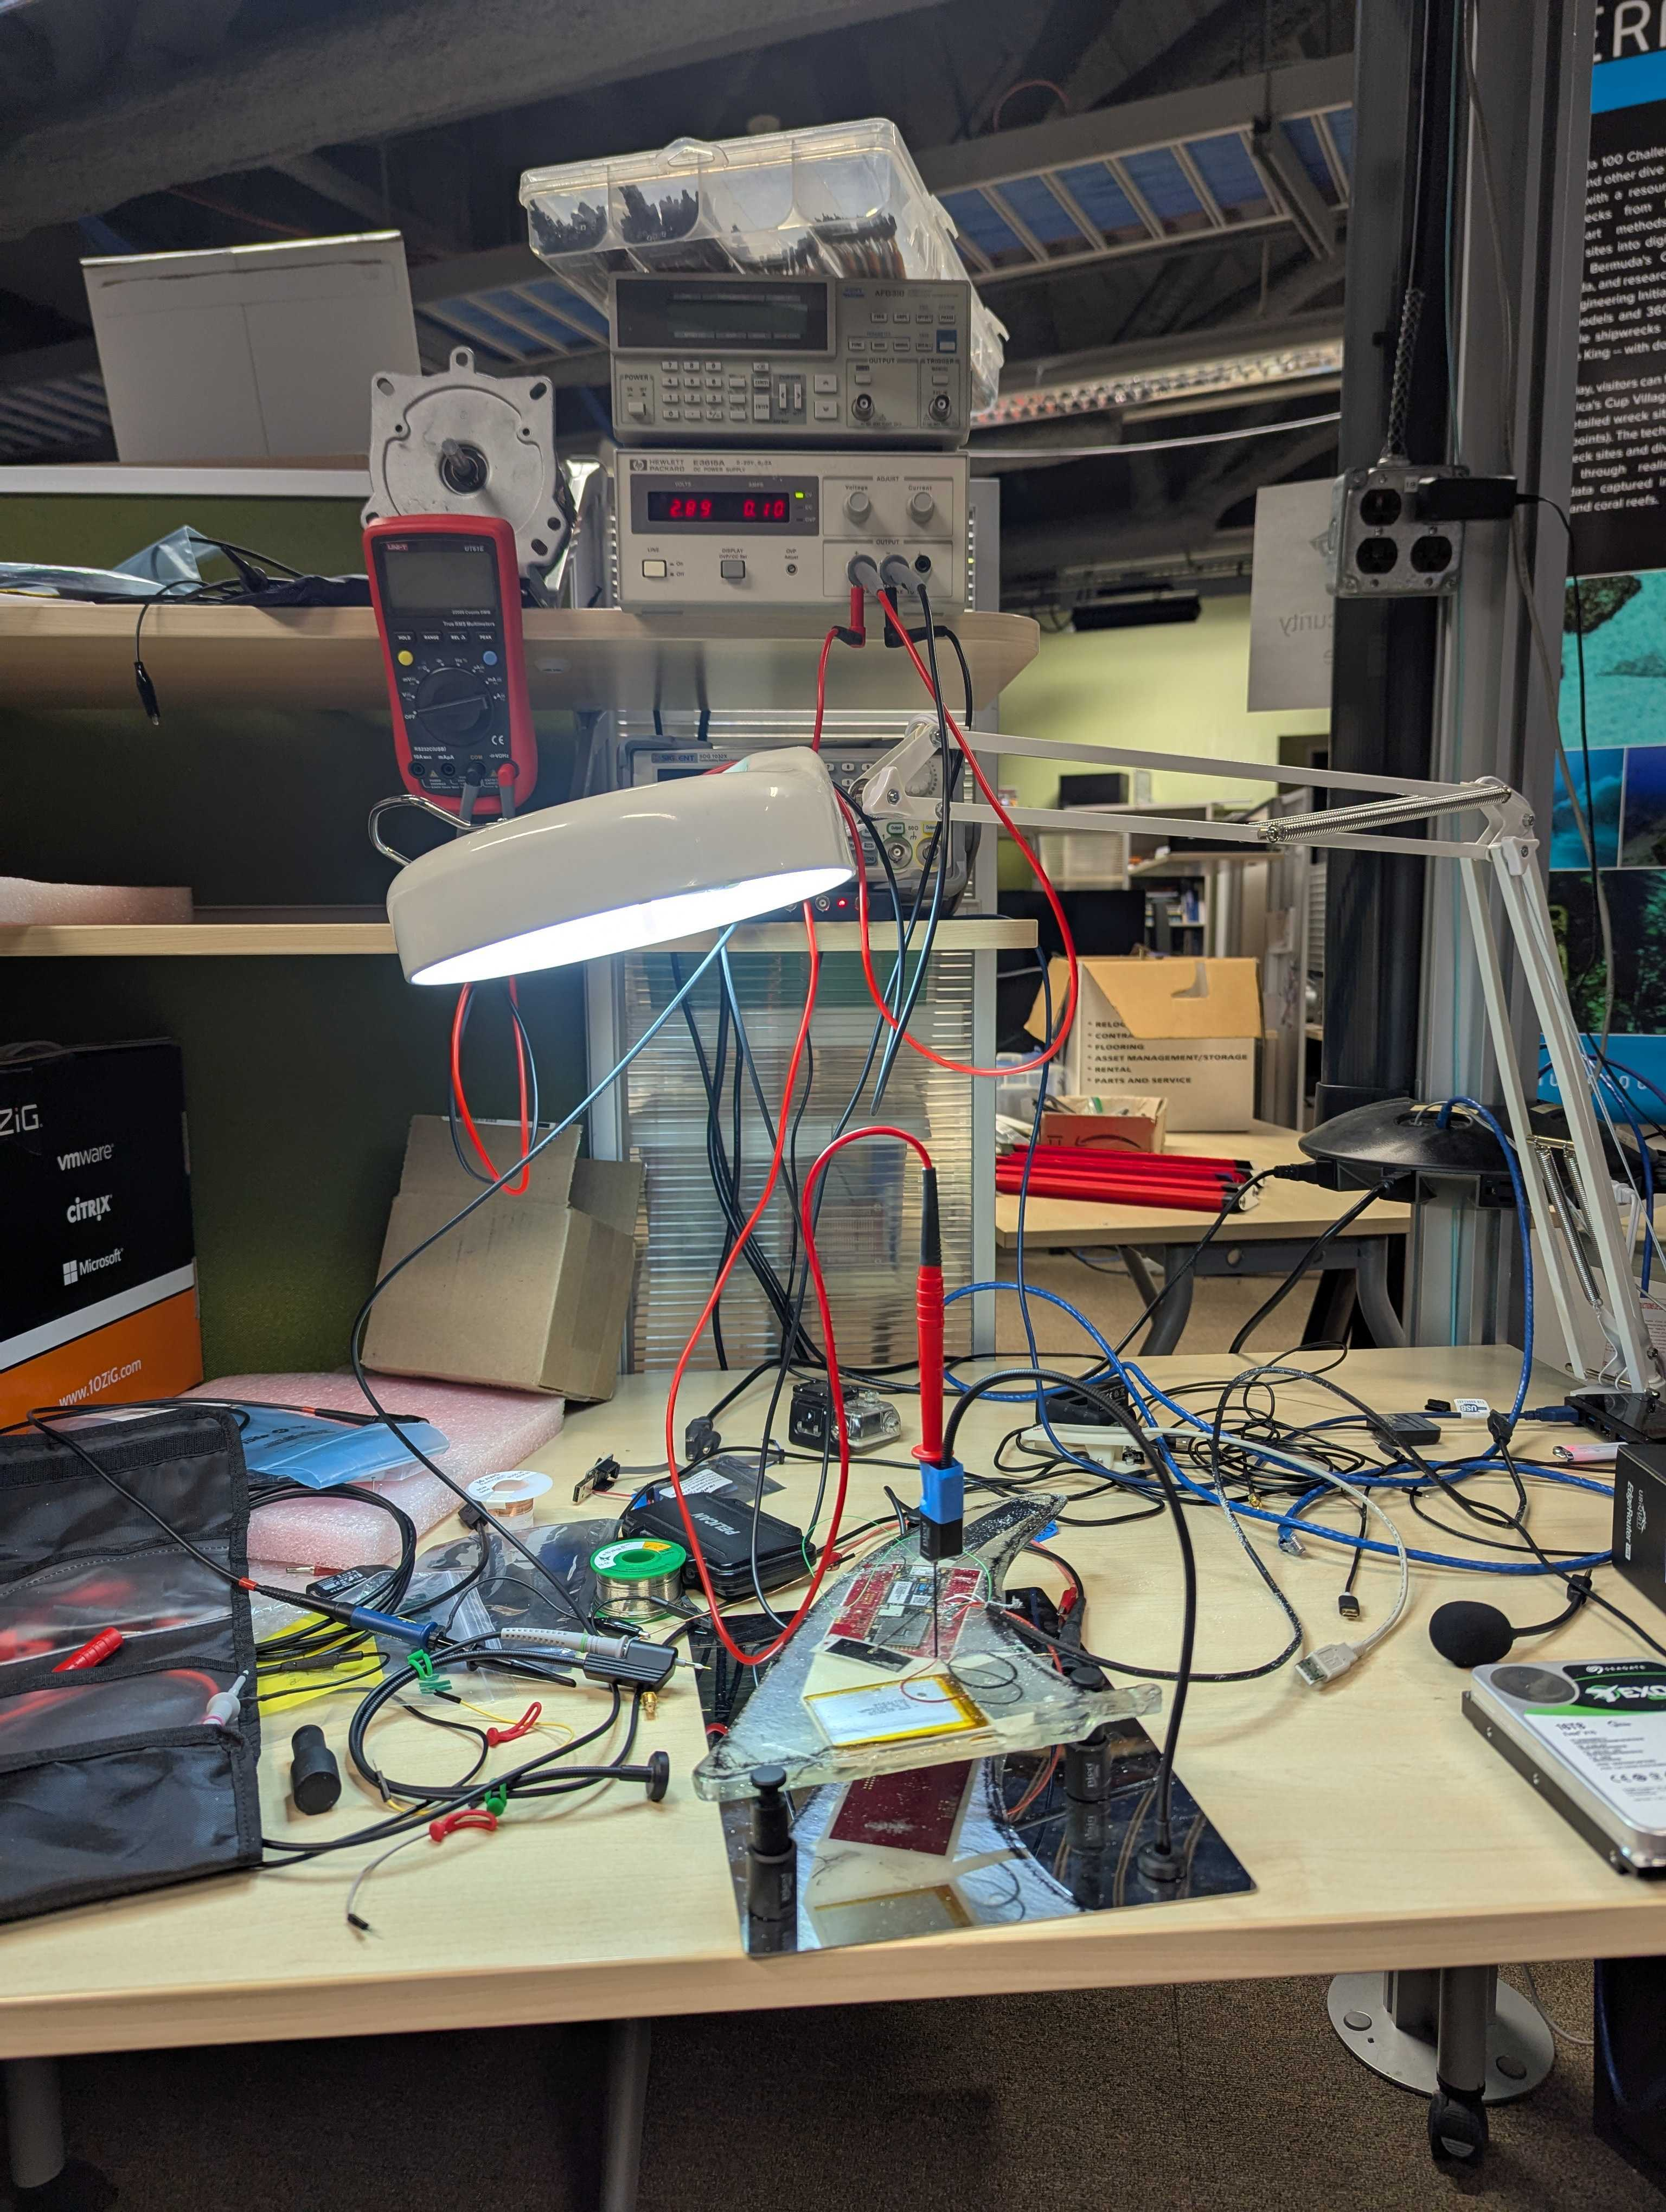
\includegraphics[height=0.6\textheight,width=0.5\textwidth,keepaspectratio]{images/sf_battery_charge_setup.jpg}    
    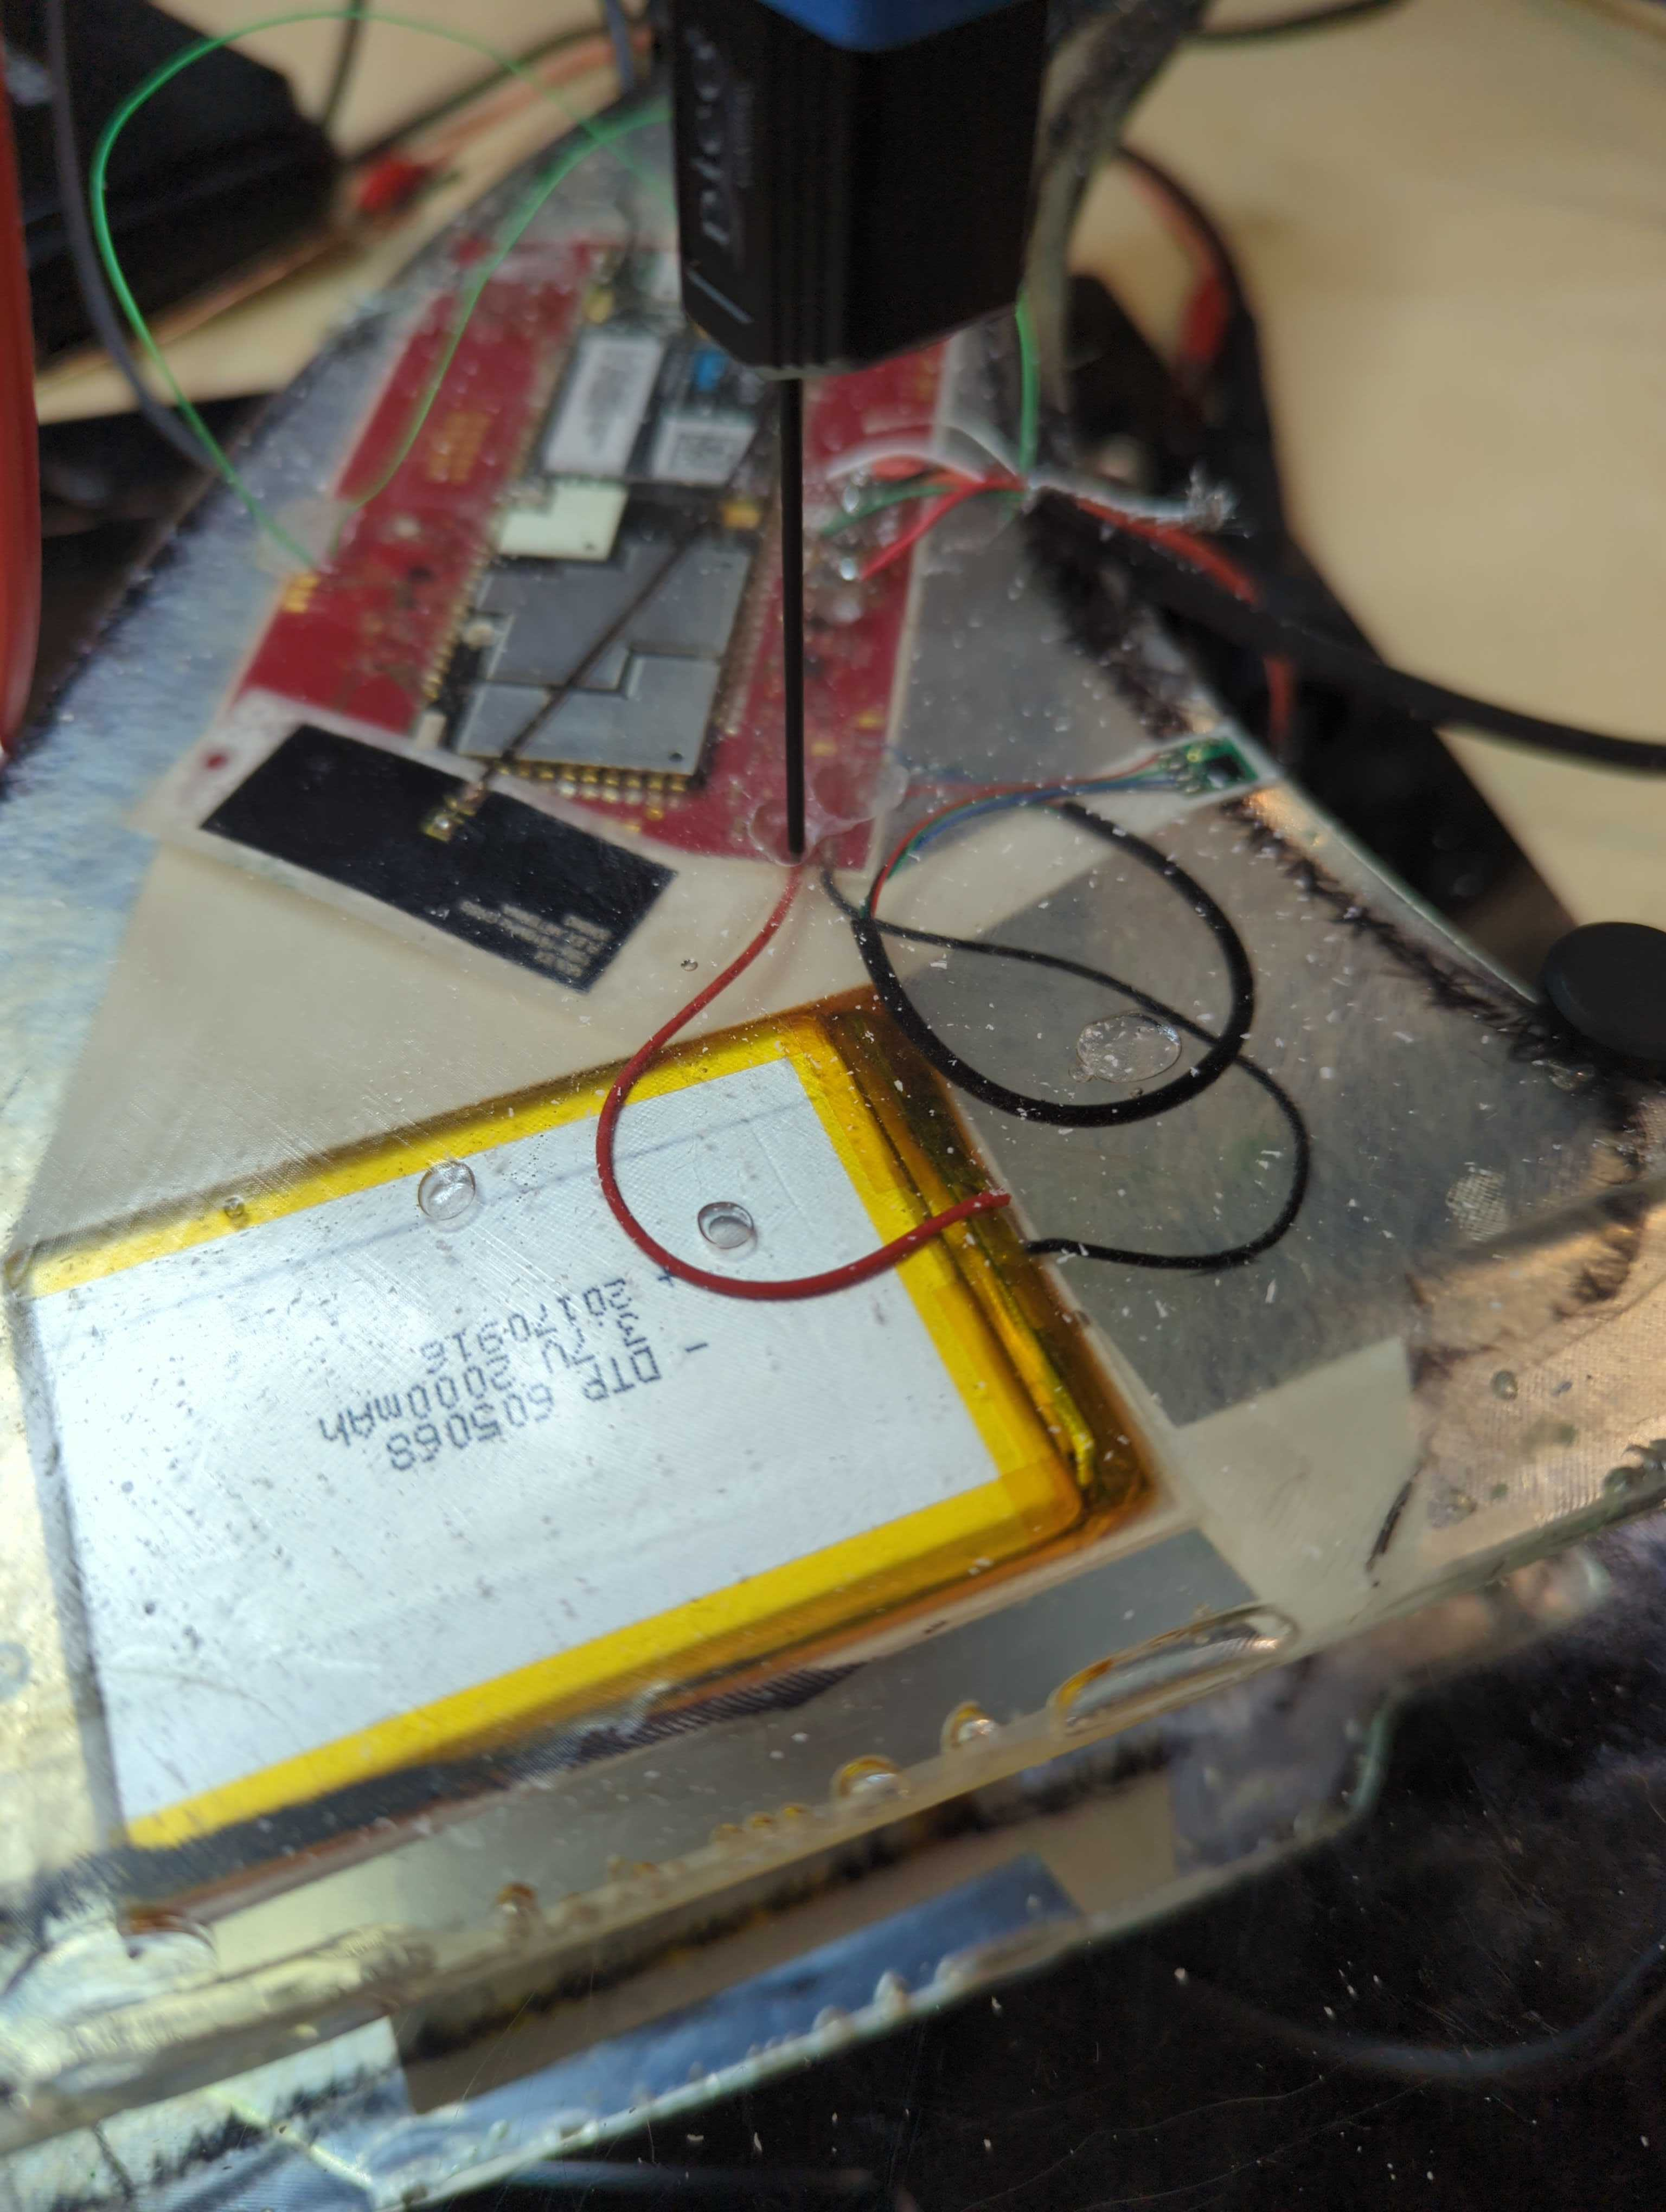
\includegraphics[height=0.6\textheight,width=0.5\textwidth,keepaspectratio]{images/sf_battery_connection.jpg}    
\end{frame}
